\documentclass[lang=cn,11pt,a4paper,cite=authoryear,twocolumn]{elegantpaper}

% 微分号
\newcommand{\dd}[1]{\mathrm{d}#1}
\newcommand{\pp}[1]{\partial{}#1}

% FT LT ZT
\newcommand{\ft}[1]{\mathscr{F}[#1]}
\newcommand{\fta}{\xrightarrow{\mathscr{F}}}
\newcommand{\lt}[1]{\mathscr{L}[#1]}
\newcommand{\lta}{\xrightarrow{\mathscr{L}}}
\newcommand{\zt}[1]{\mathscr{Z}[#1]}
\newcommand{\zta}{\xrightarrow{\mathscr{Z}}}

% 积分求和号

\newcommand{\dsum}{\displaystyle\sum}
\newcommand{\aint}{\int_{-\infty}^{+\infty}}

% 简易图片插入
\newcommand{\qfig}[3][nolabel]{
  \begin{figure}[!htb]
      \centering
      \includegraphics[width=0.6\textwidth]{#2}
      \caption{#3}
      \label{no :#1}
  \end{figure}
}

% 表格
\renewcommand\arraystretch{1.5}

% 日期

\newcommand{\homep}[1]{\section*{Problem #1}}
\newcommand{\subhome}[1]{\subsection*{SubProblem #1}}

% MATLAB 代码块环境

% \usepackage{ctex}
\usepackage[numbered,framed]{matlab-prettifier}

\lstset{
  language = octave,
  style = Matlab-editor,
  basicstyle = \mlttfamily,
  escapechar = ",
  mlshowsectionrules = true,
}
% 
% \newenvironment{ocode}{\begin{lstlisting}[language=octave]}{\end{lstlisting}}

\lstnewenvironment{ocode}[1][]{%
    \lstset{language=octave,#1}}{}%


\title{微电子器件物理\quad 第六周作业}
\author{范云潜 18373486}
\institute{微电子学院 184111 班}
\date{\zhtoday}

\begin{document}

\maketitle

% 作业内容:

% \tableofcontents

% Start Here

% End Here

\homep{单项选择}

(1) a (2) e (3) b (4) c (5) d 

\homep{2}

\subhome{1a}

\(n_i \exp ((E_i - E_F)/kT) = N_A\) 

\(\therefore\: E_i - E_F = \dfrac{kT}{1} \ln (N_A / n_i) = 0.025851 \cdot \ln 10^7 = 6.6750e-20 J\)

\(\Phi_F = \dfrac{E_i-E_F}{q} = 0.41667 V \)

\subhome{b,c,d,e}

这是 pMOS ,分别对应耗尽、积累、平带与耗尽反型转换,如 \figref{01}

\begin{figure}
    \centering
    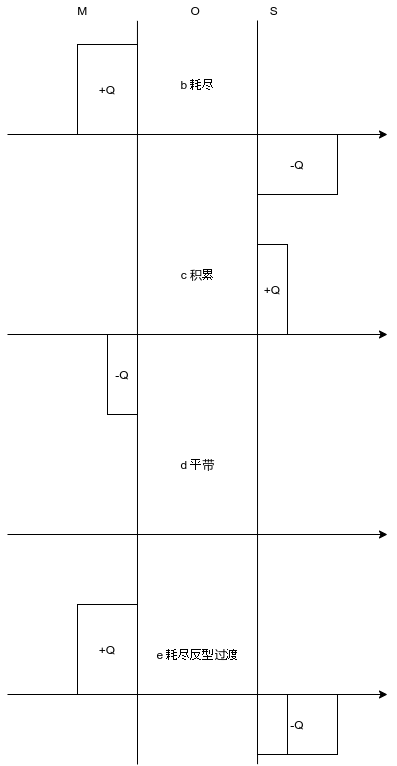
\includegraphics[width=0.4\textwidth]{h601.png}
    \caption{1 题图解}\label{01}
\end{figure}

\homep{2}

\subhome{2a} 

\(\Phi_F =  \dfrac{kT}{q} \ln (N_A / n_i) = 0.47619 V \)

\subhome{2b}

\(W = \sqrt{2 \kappa_s \epsilon_0 \Phi_S / q N_A} = \sqrt{2 \cdot 11.8 \cdot 8.85e-14 \cdot 2 \Phi_F / q N_A} = 0.0000035237 cm = 0.035237 \mu m\)


\subhome{2c}

\(E_S = \frac{q N_A W}{\kappa_s \epsilon_0} = 5.41e5 V/cm\) 

\subhome{2d}

\(V_T = V_G = \Phi_F + \frac{\kappa_S}{\kappa_O}x_0 E_S = 0.47619 + 11.8/3.9\cdot(5.41e5 \cdot 2e-7) = 0.80356 V\)

\homep{3}

\subhome{3a}

\(\Phi_S = E(0) * x / 2 = 0.240185 V\)

\[N_D = E_S^2 K_S \epsilon_0 / (2 q \Phi_S) = 1.987e17 / cm^3\]






\end{document}